\chapter{Evaluating capacitive proximity sensors in smart environments}
\label{ch:eval}
In the previous sections we have presented back-ground information on capacitive proximity sensors and various prototypes of this technology in different application domains within smart environments. In the following section we are building on the collected information to perform a meta-analysis of the acquired data, discussing benefits and limitations of the technology, compare it to competing technologies and give some guidelines to parties interested in developing further applications in this domain. 
\section{Classification of capacitive proximity sensors}
Classification
\section{Comparison to other sensing technologies}

% Table generated by Excel2LaTeX from sheet 'Tabelle1'
\begin{table}[htbp]
  \centering
  \footnotesize
  \caption{Add caption}
    \begin{tabularx}{\linewidth}{Xp{4cm}XXXX}
    \toprule
    \textbf{Name} & \textbf{Application Domains} & \textbf{Environmental Influences} & \textbf{Detection Range} & \textbf{Processing Complexity} & \textbf{Unobtrusiveness} \\
    \midrule
    \textbf{Capacitive proximity sensing} & indoor localization, smart appliances, physiological sensing, gestural interaction & electric fields, conductive objects & near distance   (< 100cm) & Few high dynamic range data sources  & invisible integration possible \\ \addlinespace
    \textbf{Capacitive touch sensing} & smart appliances, physiological sensing, gestural interaction & electric fields, conductive objects & touch  & Few binary sensors & thin cover above electrodes \\ \addlinespace
    \textbf{RGB cameras } & indoor localization, smart appliances, physiological sensing, gestural interaction & occlusion, external lights & far distance     (> 10m) & Complex image processing based on resolution & pinhole lenses \\ \addlinespace
    \textbf{Infrared cameras} & indoor localization, physiological sensing, gestural interaction & occlusion, external infrared light & medium distance (< 5m) & Complex image processing based on resolution & infrared source and camera \\ \addlinespace
    \textbf{Ultrasound sensing} & indoor localization, smart appliances, gestural interaction & acoustic occlusion, absorbing materials & medium distance (< 5m) & Few low dynamic range data sources & emitter and senders with exposed pinhole speaker, microphone \\ \addlinespace
    \textbf{Microphone arrays} & indoor localization, smart appliances, physiological sensing & environmental noise, absorbing materials & medium distance (< 5m) & Very high dynamic range data sources & exposed pinhole microphones \\ \addlinespace
    \textbf{Radiofrequency sensing} & indoor localization, smart appliances, gestural interaction & other RF devices & far distance     (> 10m) & Few low dynamic range data sources & hidden emitters and senders possible \\
    \bottomrule
    \end{tabularx}%
  \label{tab:addlabel}%
\end{table}%



In order to properly place capacitive proximity sensing in the smart environment domain it is neces-sary to include a comparison to other sensing tech-nologies. We have chosen systems that have a broad applicability and have been used in various smart environment applications. A short overview can be found in Table 7. We have included a comparison of application domains, environmental influences, de-tection range, processing complexity and unobtru-siveness of the technology. 
Capacitive touch sensing, as opposed to capacitive proximity sensing relies on an electrode being touched instead of an object being in proximity and is ubiquitous in touch screen applications.
RGB cameras are a class of image sensors operating in the same frequency domain as the human eye. They are capable of processing different colors.
Infrared cameras operate in near light frequencies that are invisible to the human eye. This allows for application in dark environments and we can project infrared light into the scene without disturbing the user.
Ultrasound sensing is using a low frequency range just above the audible limit of human hearing. The waves propagate similar to sound signals and we can perform reflection measurements or time-of-flight methods.
Microphone arrays detect signals in the range of human hearing, and thus work with audible signals, such as human speech.
Radiofrequency (RF) sensing uses signals in a range between several hundred kHz up to 5GHz, typically used for wireless communication. Commonly the signal strength or time of flight is used to gather information about the environment.
Most technologies are capable of supporting multiple application domains. Some non-intuitive examples include WiSee that enables whole-body gestural interaction using WiFi signals [86] or MoGees that uses a single microphone to enable gesture interfaces on various surfaces [87]. 
Capacitive sensors are disturbed by conductive objects and electric fields, whereas cameras struggle with occlusion and additional light sources. Occlusion is a weak point, and a line of sight is required. Sound sensors are prone to dampening materials and environmental noise interfering with the signal. RF signals usually propagate well through most materials and only external sources may be an issue. 
The detection range of the technologies varies strongly. RF ranges before light, sound and electric fields. However, this again strongly depends on apxplication and layout of the sensing devices.
It is not easy to find a good measure about the processing complexity associated to a different sensing technology. We are using a simplified model, taking the dynamic range of a sensor and the number of sensors typically required. Dynamic range is the difference between the smallest detectable value and the largest detectable value. Microphones have a high dynamic range measuring over a larger frequency scale, whereas touch sensors only have two different states. 
Finally capacitive sensors and RF sensors can be applied completely invisible. Cameras, microphones and ultrasound need a direct connection to the out-side world. However, there are very small variants available that are barely visible to the naked eye.


\section{Limitations}
Despite the potential benefits that have been outlined in the previous section, capacitive proximity sensors have a number of limitations that may hinder several applications. 
Similar to the benefits I am putting these into three different groups that are outlined in Table \ref{tab:cap_limitations}. Environmental influences have been briefly mentioned throughout this work and have to be considered in any setup. The physical range limits the object detection to a low distance from the sensing electrode. The objection detection similarly suffers from the physical limitations of electric field sensing. These three groups will be detailed in the following paragraphs.

\begin{table}[htbp]
  \centering
  \caption{Overview of capacitive proximity sensing limitations}
    \begin{tabular}{p{4cm}p{6cm}}
    \toprule
    \textbf{Name} & \textbf{Examples} \\
    \midrule
    \textbf{Environmental influence} & Static electric fields, dynamic electric fields, temperature, humidity, conductive objects \\
    \textbf{Physical range} & Small differences in capacitance, reduction due to influences, physical limitations \\
    \textbf{Object detection} & Small number of data points, a priori knowledge \\
    \bottomrule
    \end{tabular}%
  \label{tab:cap_limitations}%
\end{table}%

\subsection{Environmental Influence}
One of the main limitations of capacitive proximity sensors is their sensitivity towards environmental influences. Any factor that modifies an electric field will also affect the measurement of a capacitive sensor. The current environmental parameters, like temperature and humidity are having a considerable effect on the medium in which the electric field propagates. However, those changes are usually over a longer period of time and can be compensated using a factor for drift, as described in the previous sections about noise reduction. While the frequency range in which the sensors operate is usually not in an interval that disturbs other electronic systems, there are some electromagnetic sources in the environment. The most common  are power supplies (frequency range of 50-60 Hz) terrestrial radio (frequency range of 150 kHz to 100 MHz), mobile phone communication (870-970 MHz and 1700-1900 MHz), as well as WiFi (2,4GHz and 5GHz). While in theory there is some potential interference with the terrestrial radio spectrum, the effect is fairly small and can be covered by choosing intermediate frequency intervals. Thus it is feasible to use capacitive sensing even in environments, where non-disturbance is a main requirement.

The main source of disturbance occurring in our evaluations, was the influence of very close electromagnetic sources and disturbing signals within the power grid. One example for a disturbing source was a plasma TV installed in our Living Lab. When turned on the CapFloor prototype (\ref{ch:prot_capfloor}) suffered from severe noise, preventing any successful tracking of persons. The culprit are high frequency internal power supplies that drive the plasma cells. Newer TVs are using different internal electronics that significantly reduce the emitted electric field. Another disturbing factor can be faulty power supplies that are attached to the grid and produce frequency noise. As this noise typically operates in a limited frequency range, it is possible to use frequency domain filtering that attenuates these bands. Thus, it should be attempted to apply capacitive proximity sensing in an environment that adheres to all relevant standards regarding electromagnetic compliance. Additionally, the systems should be designed in a way that reduces potential external influences, e.g. by using internal power supplies that are stabilized and applying shielding where necessary. 
 
An additional issue might arise when placing sensors close to each other. The created electric fields may disturb the measurement if some electrodes are charged and create fields to adjacent electrodes while those are discharged for measurement. This is particularly challenging, when a larger number of sensors is involved. Here, this is the case for the CapFloor (\ref{ch:prot_capfloor}) and CapTap (\ref{ch:prot_captap}) prototypes. In the case of CapTap specific charge-discharge cycles for the electrodes are used that ensure that adjacent sensors are not interfering with each other. Similarly the CapFloor attempts to control the sensors in a way that prevents interference, taking into account the geometric layout and the position of the electrodes within the area. Both methods are a form of multiplexing that is based on time (TDMA). Other options include a variety of different multiplexing methods, such as the previously mentioned frequency method of Honeyfish (\ref{ch:prot_otherprot}). Code division multiplex is a last class of multiplexing methods that relies on the modification of the signal. This was employed by the presented capacitive sensor of Rob MacLachlan \cite{MacLachlan2004}. It can result in very precise measurements, but requires specialized hardware. Thus, it was not used in any of the developed prototypes.

Another major challenge are conductive objects that are permanently placed in the immediate sensing environment. It is difficult to distinguish the object we want to detect from a disturbing object, if their influence on the electric field is similar. Long term data analysis may help in performing a successful detection. The CapTap prototype, as a regular living room table, should not fail when disturbing objects are present, such as glasses full of water (\ref{ch:prot_captap}). This can be achieved by performing a feature analysis that detects the typical response of the disturbing object and performs a recalibration that takes the object into account. 

The CapFloor prototype is affected by environmental influences the most, given the small size of the electrodes relative to the interaction area and the changing environment on top of the floor (\ref{ch:prot_capfloor}). Strong noise reduction algorithms and drift compensation are used to create a more stable result that however causes a reduction of the detection range.
\subsection{Physical Range}
\begin{figure}[ht]
\centering
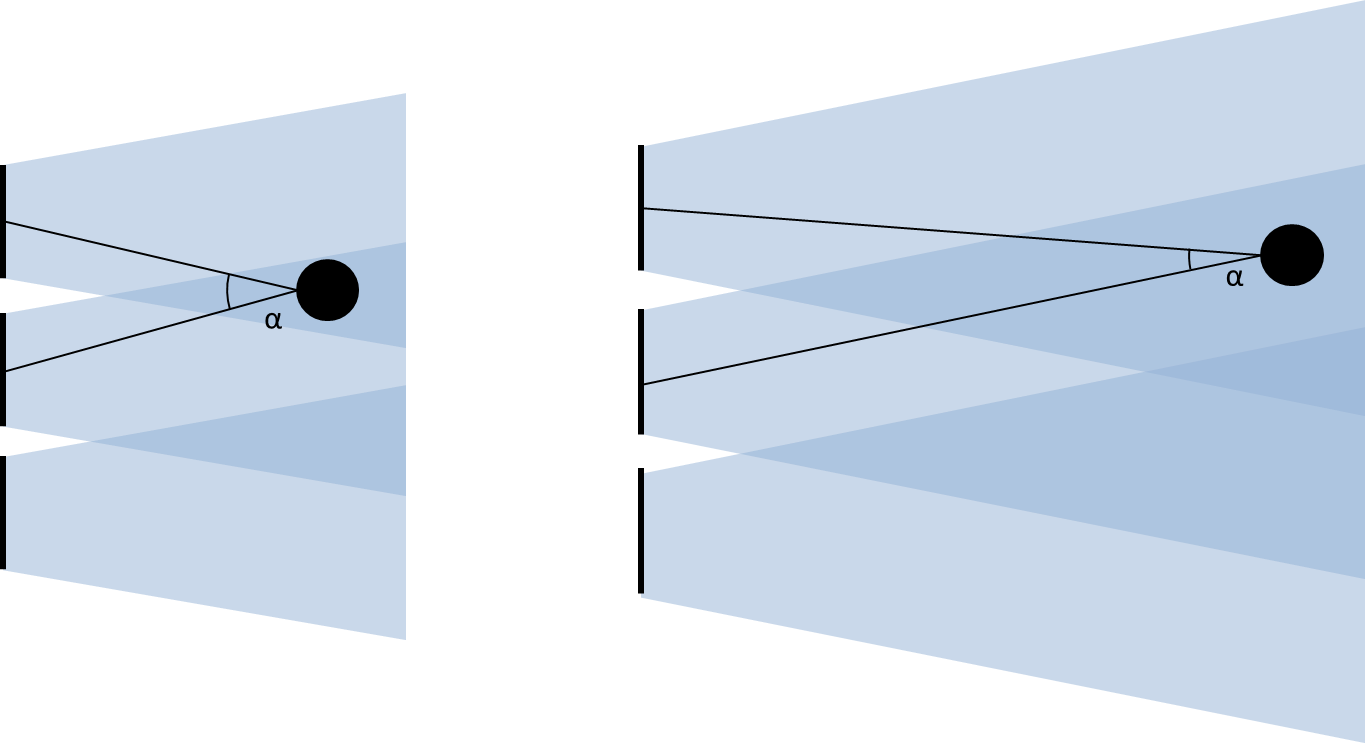
\includegraphics[width=0.8\textwidth]{images/limit_distance}
\caption{Reduced angular resolution on smaller, distant objects}
\label{fig:disc_ang_resolution}
\end{figure}

The physical range of the generated electric field is one of the main limiting factors of capacitive proximity sensing. In order to detect objects that are further away,  the electric field strength has to be increased sufficiently. This is easier for larger electrodes, as its potential capacitance is higher. However, this also leads to distant objects having an ever smaller influence on the overall capacitance. In this case we need more precise measurement circuits and longer measurement times to improve the signal-to-noise ratio. Additionally, looking at smaller objects the angular resolution will decrease as shown in Figure \ref{fig:disc_ang_resolution}. This makes it more difficult to get a precise localization as the immanent noise leads to an angular error. While this can be compensated using more sensors, the far distance would require us to use large electrodes that have to be placed further apart resulting in a huge area that would have to be equipped with sensor electrodes. The Capacitive Chair prototype uses large electrodes that allow us to detect the presence of a person at distances of around 50-60 cm (\ref{ch:prot_capchair}). It is designed to detect whole body parts and thus does not need any fine resolution. The Active Armrest on the other hand has a finger interaction array comprised of small electrodes that have a detection limit of approximately 15 cm (\ref{ch:prot_armrest}). Yet, it is able to detect fine movements and precise locations of the fingers within this range.

In general, the achievable resolution is not comparable to vision based system and has to be taken into consideration when designing the specific application. A balance between electrode size, physical range and achievable resolution has to be found. The MagicBox size does not allow an integration of very large electrodes (\ref{ch:prot_magicbox}). Instead, we are optimizing the available space in order to achieve a detection that lets us detect hands in a distance of approximately 30 cm and allows reliable tracking in distances between 15 and 20 cm. The system with the lowest detection distance is the CapFloor prototype (\ref{ch:prot_capfloor}). The long wire electrodes are not particularly well suited for achieving a good resolution and are prone to interference. However, they are suitable for this specific purpose and objects at a proximity of 10 cm or less can still be detected. 

\subsection{Object Detection}
\begin{figure}[ht]
\centering
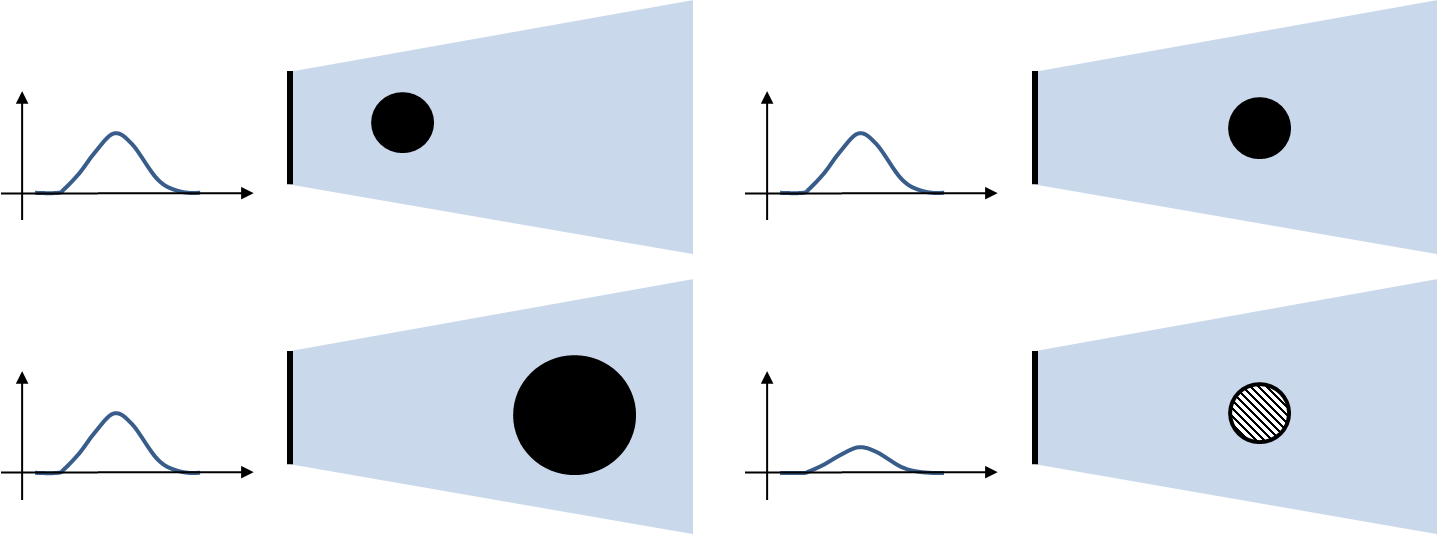
\includegraphics[width=0.8\textwidth]{images/limit_detection}
\caption{Same response to differently sized objects (left), different response to varying materials (right)}
\label{fig:disc_obj_detection}
\end{figure}

Object detection using capacitive sensors, can be partially compared to object detection using camera systems, with a single sensor being equivalent to a single photo sensor. Smith et al. propose that loading mode measurements resemble light captured by a camera without a lens, as only one part of the electric system is constrained \cite{smith1998electric}. The light intensity measure is comparable to field intensity and likewise it is not possible to distinguish if the measurement is caused by a weak source in close proximity or a strong source at a further distance. As a practical example the capacitive sensor is not able to decide if one hand is close to the sensor or two hands are a bit further away. This effect makes it challenging to provide object detection and usually information from various sensors has to be combined to get a good idea about object shape and size. The CapTap prototype is able to detect two hands by combining the information of 24 sensors and additionally uses an analysis of the arm posture in the detection area (\ref{ch:prot_capfloor}). Due to the presented challenges in physical range and electrode size, capacitive proximity sensing systems do not have the same level of scalability as cameras, where millions of photo sensors can be placed in very small areas. Touch screens show that capacitive sensing technology has a very high resolution in near ranges. However, this can't be translated to similar resolution in further distances.

Additionally, the effect of an object on the electric field is not always closely correlated to the object dimensions, but instead based on conductivity, material and other factors. The same response to different objects may be measured at different distances, if they are differently sized or are made of different materials, as shown in Figure \ref{fig:disc_obj_detection}. In the presented application scenarios exclusively parts of the human body are tracked. Mostly, there is also an assumption that no other objects should be used. The CapTap will have to identify potential foreign objects from the hands of the user (\ref{ch:prot_captap}). In this case, the specific capacitance profile of objects at close proximity can be used, similar to the capacitance tags presented by SmartSkin \cite{rekimoto2002smartskin}. The Active Armrest has gestures for one and two fingers that are distinguished using a simple threshold (\ref{ch:prot_armrest}). If another object is entering the field, or the person is having a strongly different finger size, the system will fail to properly differentiate gestures. Accordingly, some other compensation methods should be used.


\section{Benefits}
Given the information collected in the previous section I can now discuss the specific benefits of capacitive proximity sensing. I am using three different groups for categorization, namely versatility, unobtrusiveness and processing complexity. Some examples within these groups are shown in Table \ref{tab:cap_benefits}. In the following section I will discuss those groups in detail.

\begin{table}[htbp]
  \centering
  \caption{Overview of capacitive proximity sensing benefits}
    \begin{tabular}{p{4cm}p{6cm}}
    \toprule
    \textbf{Name} & \textbf{Examples} \\
    \midrule
    \textbf{Versatility} & Flexible electrode design, scalability, different sensing methods \\
    \textbf{Unobtrusiveness} & Invisible application, non-disturbing frequency range \\
    \textbf{Processing Complexity} & Small number of sensors, variable dynamic range \\
    \bottomrule
    \end{tabular}%
  \label{tab:cap_benefits}%
\end{table}%

\subsection{Versatility}
A main benefit of capacitive proximity sensors is the versatility in which they can be applied. With flexible choice of electrode materials, size and geometry it is possible to create highly individual applications. Some example electrodes include transparent metal oxide layers, woven conductive thread, copper wires, PCB boards, or simple aluminum foil. In the different prototypes I have used a large variety of materials, including aluminum foil in the MagicBox (\ref{ch:prot_magicbox}), long copper wire electrodes in the CapFloor (\ref{ch:prot_magicbox}), conductive thread in the Capacitive Chair (\ref{ch:prot_magicbox}), and transparent ITO in GestDisp (\ref{ch:prot_otherprot}). Other materials in the literature include plant tissue for Botanicus Interactus \cite{poupyrev2012botanicus} and water in Touché \cite{Sato2012}. The size and shape of the electrodes is varying accordingly. The finger tracking array in the Active Armrest (\ref{ch:prot_armrest}) consists of 2 cm x 3 cm copper PCB, while the Capacitive  Chair (\ref{ch:prot_capchair}) has some electrodes of 15 cm x 20 cm. The largest electrodes of the related works can be found in the TileTrack prototype using 60 cm x 60 cm tiles \cite{valtonen2010human}. The electrode design can be modified freely according to the specific application scenario. Given the large variety of different sensing methods most scenarios can be covered.

Additionally, the sensor systems are also highly scalable. By choosing appropriate voltages and frequencies it is possible to add a high number of sensors to a single object. Rekimoto's SmartSkin uses shunt mode, with nine emitters and eight receivers leading to 72 sensing points \cite{rekimoto2002smartskin}. The CapTap prototype uses three OpenCapSense boards, interfacing 24 sensors, relying on time multiplexing to prevent interference between the different sensors (\ref{ch:prot_captap}). The CapFloor prototype as used in the EvAAL competition connected 26 sensors to a single PC system, controlled by two different communication interfaces (\ref{ch:prot_capfloor}). Further iterations developed by Tobias Grosse-Puppendahl support more than one hundred sensors in setups covering multiple rooms. Using smart measurement windows and different multiplexing methods, sensors can be placed close together and electrodes may act as both sender and receiver, e.g. the frequency multiplexing method used in the Honeyfish system \cite{grosse2012honey} (\ref{ch:prot_otherprot}). The different sensing methods presented - loading mode, shunt mode and transmit mode, enable a variety of different sensing patterns. The human body can be used as both sender and receiver and smart electrode layouts allow using low-powered processors. 

In conclusion, it is possible to add capacitive sensing to most everyday objects to enable different forms of interaction, create natural interfaces and smart objects. The developed prototypes are using different electrode materials, flexible or solid electrodes, conductive thread, wires, shielded or non-shielded layouts.
 
\subsection{Unobtrusiveness}
\begin{figure}[ht]
\centering
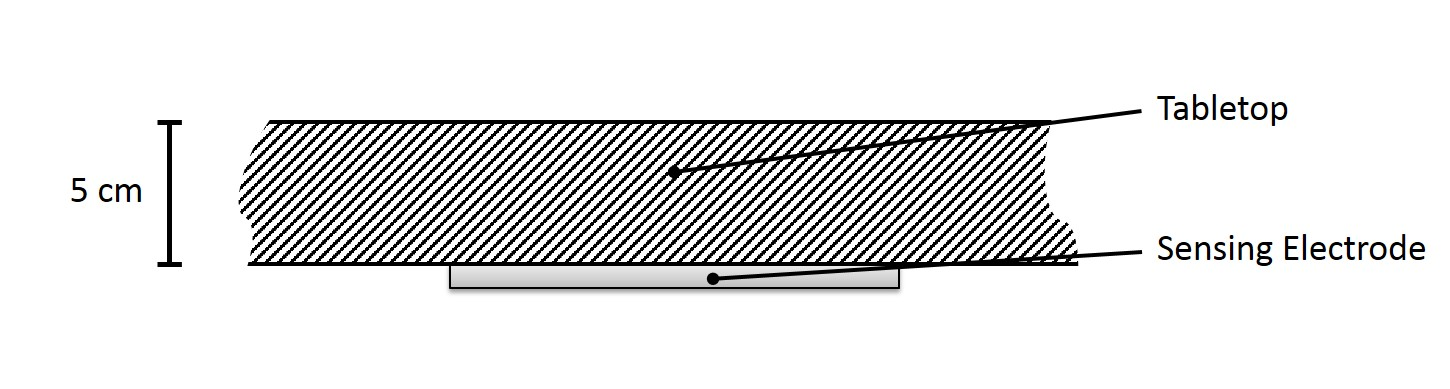
\includegraphics[width=0.8\textwidth]{images/eval_unobtrusive}
\caption{Sketch of CapTap prototype showing thickness of tabletop}
\label{fig:eval_unobtrusive}
\end{figure}

Electric fields are not usually perceived by persons, unless they are of exceptional strength. Capacitive proximity sensors usually operate with low voltages (OpenCapSense operates at 3.3 V or 5 V) and with frequencies that are not considered biologically active (OpenCapSense uses a 100 kHz sampling rate). Furthermore, they propagate through many materials that are typically present in our environment, including most plastics, wood or tile. This allows to invisibly apply capacitive proximity sensors without a strong effect on the measurement. Regarding the Smart Bed, (\ref{ch:prot_smartbed}) the signal propagates through a thick layer of mattress, consisting of polyurethane foam. The CapFloor system is designed to work below wood, PCV, tile, or other non-conductive floor materials (\ref{ch:prot_capfloor}). An application below several centimeters of covering is possible, if the electrodes are designed properly for large distance sensing. The detection range of the CapTap demonstrator is not disturbed by the laminated wood tabletop of 5 cm thickness (\ref{ch:prot_captap}). Similar the Capacitive Chair has electrodes attached below a cover comprised of wood, polyurethane foam and cloth, the materials of the seat area (\ref{ch:prot_capchair}). Other materials that were applied above capacitive proximity sensors in the scope of the experiments were glass, polycarbonate, carpet, or access floors that are comprised of a wood, plastic and carpet combination. None of the materials we used showed unexpected behavior, related to absorption or attenuation of the sensor signal. If the sensors are attached close to conductive materials the signal can be disturbed if they are grounded or acting as shield towards the object to be sensed. Shielding in this context describes preventing the electric field created by the sensors to propagate to the object that is supposed to be detected, e.g. the famous Faraday cage. In some scenarios capacitive proximity sensors can also be used to detect properties of conductive objects, e.g. detecting the level of water in a glass or other non-conductive container.

It is possible to equip most conductive objects directly with capacitive proximity sensors, and hide them below non-conductive objects with minimal spatial requirements. The Active Armrest (\ref{ch:prot_armrest}) prototypes are using sensor sets that are completely invisible from the outside.  The CapTap was specifically designed to combine several sensing technologies that are invisible from the outside - hidden electrodes and a microphone (\ref{ch:prot_captap}). The thickness of the tabletop is shown in Figure \ref{fig:eval_unobtrusive}. One disadvantage of this method is the disability to easily detect touch if there is no contact between object and electrode. Touching the electrode will typically cause a spike in sensor values that can be very easily discriminated. Therefore, in order to detect touches narrow thresholds and suitable sensing electrodes have to be used, as shown in SmartSkin \cite{rekimoto2002smartskin} or the touch area of the Active Armrest (\ref{ch:prot_armrest}). Another potential solution is to use indirect effects of touching. The Smart Bed is using the pressure applied on the mattress to cause a geometric deformation of the electrode (\ref{ch:prot_smartbed}). This results in a clearly measurable spike in sensor values and can be modified for application below other flexible surfaces.
The Smart Bed is additionally designed to communicate wireless to a PC, only using a regular power supply for operation.
 
\subsection{Processing Complexity}
An appropriate analogy to capacitive proximity sensors is a single photo diode. As opposed to a light intensity, capacitance is measured. While the information we can gain from such a measurement is limited, the processing required to analyze the signal is also low. Performing signal analysis on an array of 24 capacitive sensors, as in the CapTap prototype (\ref{ch:prot_captap}) is comparable to processing the image of a 6x4 pixel camera. Therefore, it is easy to create highly integrated systems with low-power devices for performing any subsequent data analysis. Other prototypes use even less electrodes, most notably the Magic Box that uses only six sensors and computationally inexpensive object localization algorithms (\ref{ch:prot_magicbox}). 

While it is in many cases beneficial to use complex data processing algorithms for object detection, it is often possible to achieve a similar result with less complex methods. In many applications it is even viable to opt for a quantized capacitance measurement. In the case of a touch sensor a single binary measure is sufficient. However, it is also possible to select various different levels. The Active Armrest processes the two back electrodes in a quantized fashion, just using a single threshold for each (\ref{ch:prot_armrest}). The sensor dynamic can be reduced to any suitable range, thus reducing the processing complexity later in the algorithms. The CapFloor system uses a larger number of sensors and does not require a high dynamic range for calculations  (\ref{ch:prot_capfloor}) and thus uses shortened 4 Bit values.

With the exception of the Capacitive Chair (\ref{ch:prot_capchair}) and the CapTap (\ref{ch:prot_captap}) that make extensive use of frequency domain operations, our prototypes are using simple data processing methods that can be easily applied on embedded systems. One of the presented examples is the weighted average algorithm for object detection, as shown for the Magic Box (\ref{ch:prot_magicbox}). Regarding model-based data processing, even very simple cylindrical models, such as the one used for the Smart Bed (\ref{ch:prot_smartbed}), are capable to reliably predict numerous postures that are relevant in real world applications. In general, the low requirements for data pre-processing, allows dedicating more resources to high-level data processing algorithms if the specific application is resource constrained. Thus, it is easily possibly to fuse the data of multiple heterogeneous sensors in the system or apply more complex classification methods, such as the SVM classifier used for the Capacitive Chair (\ref{ch:prot_capchair}).

Another option to reduce the processing load is reducing the sample rate of the sensors. If this is done in hardware, there is an additional benefit to this method. The sensitivity of the sensors can be increased, as loading and unloading times can be decreased, making it easier to detect changes in the resulting capacitance. However, this method is not feasible for all electrode sizes, as particularly small electrodes will reach their capacitance limit early. Another option to increase the sensitivity is increasing the voltage, which influences the propagation range of the electric field. In this case, it is more difficult to guarantee biological inactivity and a low power consumption.

The OpenCapSense toolkit that is the base for most of the prototypes has a fairly powerful micro controller that is able to implement all of the processing steps. This enables highly integrated, low-power capacitive proximity sensing prototypes that can be used in smart environment applications. It is also viable to use low-powered PC systems, such as the Raspberry Pi, to interface a large number of capacitive proximity sensors in research applications.

\section{Guidelines}
After discussing the limitations and benefits of capacitive proximity sensors, the final section of this chapter will give some general guidelines on their application. The first step of this process is a decision if capacitive sensors technology is suitable for the given application. This part should be driven by three questions.
What do I need to measure in my application scenario?
Capacitive proximity sensors can measure the presence and properties of conductive, grounded objects. This includes the various application scenarios shown in the previous sections. However, if the application requires measuring properties of unsupported objects that are non-conductive, a different technology should be chosen.


\textit{What sensing technologies are supporting the required measurements?}


It may be the case that multiple technologies sup-port the measurements required in this specific applications. Cameras often can provide similar recognition as capacitive sensors, e.g. in indoor localization applications. In this step all potential sensing technologies should be collected.
Are capacitive proximity sensors beneficial for my scenario?
An evaluation of the different candidates is the final step and should lead to a decision about the most suitable sensing technologies. If the distance is too high for capacitive proximity sensors or enough processing power is available and lighting conditions are static, cameras might be more suitable. This should be driven by the different benefits and limitations of  the technologies.
If there is a decision in favor of capacitive sensors the next step is to design the specific electrode layout. Similar to technology selection we can use a few basic questions to get an idea of what layout to use.


\textit{How many sensors are required to get the measurement?}


The number of sensors required is depending on the area we want to cover, the specific object parameters that have to be determined and the desired resolution. The electrodes are inherently limited in size, as a single sensor can only charge and discharge to a specific maximum capacity. Therefore, if a large area has to be covered more electrodes and sensors are necessary. If we just want to measure the presence of a hand a single electrode may suffice. If orientation and position are interesting we need to combine measurements from various sensors.


\textit{What should be the size and geometry of the electrodes?}


This is closely related to the previous question. If the application is not restricting the available space, the electrode should be approximately of the same size as the object that is to be detected. This generates the highest difference in capacitance when the distance is changing. 


\textit{What is the best electrode material to use?}


Copper is always a good first choice to create electrodes. If elasticity is necessary we can use copper foil and solid copper if that is of no concern. For transparent electrodes we will have to use one of the previously presented materials, such as ITO. If electrodes have to be integrated into cloth, conductive thread is a good candidate. Any conductive material will act as an electrode, thus the application and budget should be the primary driver of this decision.


\textit{Does my application require any shielding?}


Shielding allows detecting only objects approaching from a certain direction. If the application re-quires this additional hardware, because it is anticipated that other objects might disturb the measurement, shielding should be used.
Finally, if the hardware is designed as desired the different variations of data processing have to be chosen and configured according to the application.
Using baseline calibration is beneficial in the vast majority of applications. Having a distinct starting point simplifies all further steps of high-level data processing, such as normalization and setting different thresholds. This step may only be omitted in very stable environments and if the system has sufficient a priori information to operate on raw data. Drift compensation should be handled in a similar fashion. The common methods are not computationally expensive and having a stable baseline over time allows the same algorithms to be applied in a more robust fashion. The method and configuration of noise reduction are strongly depending on the specific case. Some form of noise reduction might be required in most applications. Yet, according to the type of noise different methods can be used. If outliers are an issue a median filter is appropriate; if a smoother signal is desired an average filter can be used. 
Regarding high-level data processing there are manifold variations of methods. Data-driven machine learning algorithms are a good method if we have a small set of potential outcomes of our applications, e.g. the different postures that could be recognized on a chair or couch. If our application has many different potential outcomes, e.g. the thousands of potential locations in a hand tracking system, it is typically beneficial to use a model-driven approach. However, these models may be supported by data-driven algorithms, such as particle filters. One example is the Swiss-Cheese object tracker by Grosse-Puppendahl et al. \cite{grosse2013swiss}. The data processing examples shown in the previous sections give an idea of the decision rationale in various application domains.
We can say in conclusion that capacitive proximity sensors are a viable, or even, ideal solution for a considerable number of different applications. However, a certain level of preparation is required in the design process to create a system that benefits from the technology.
